\begin{figure}
    \centering
\begin{knitrout}
\definecolor{shadecolor}{rgb}{0.969, 0.969, 0.969}\color{fgcolor}
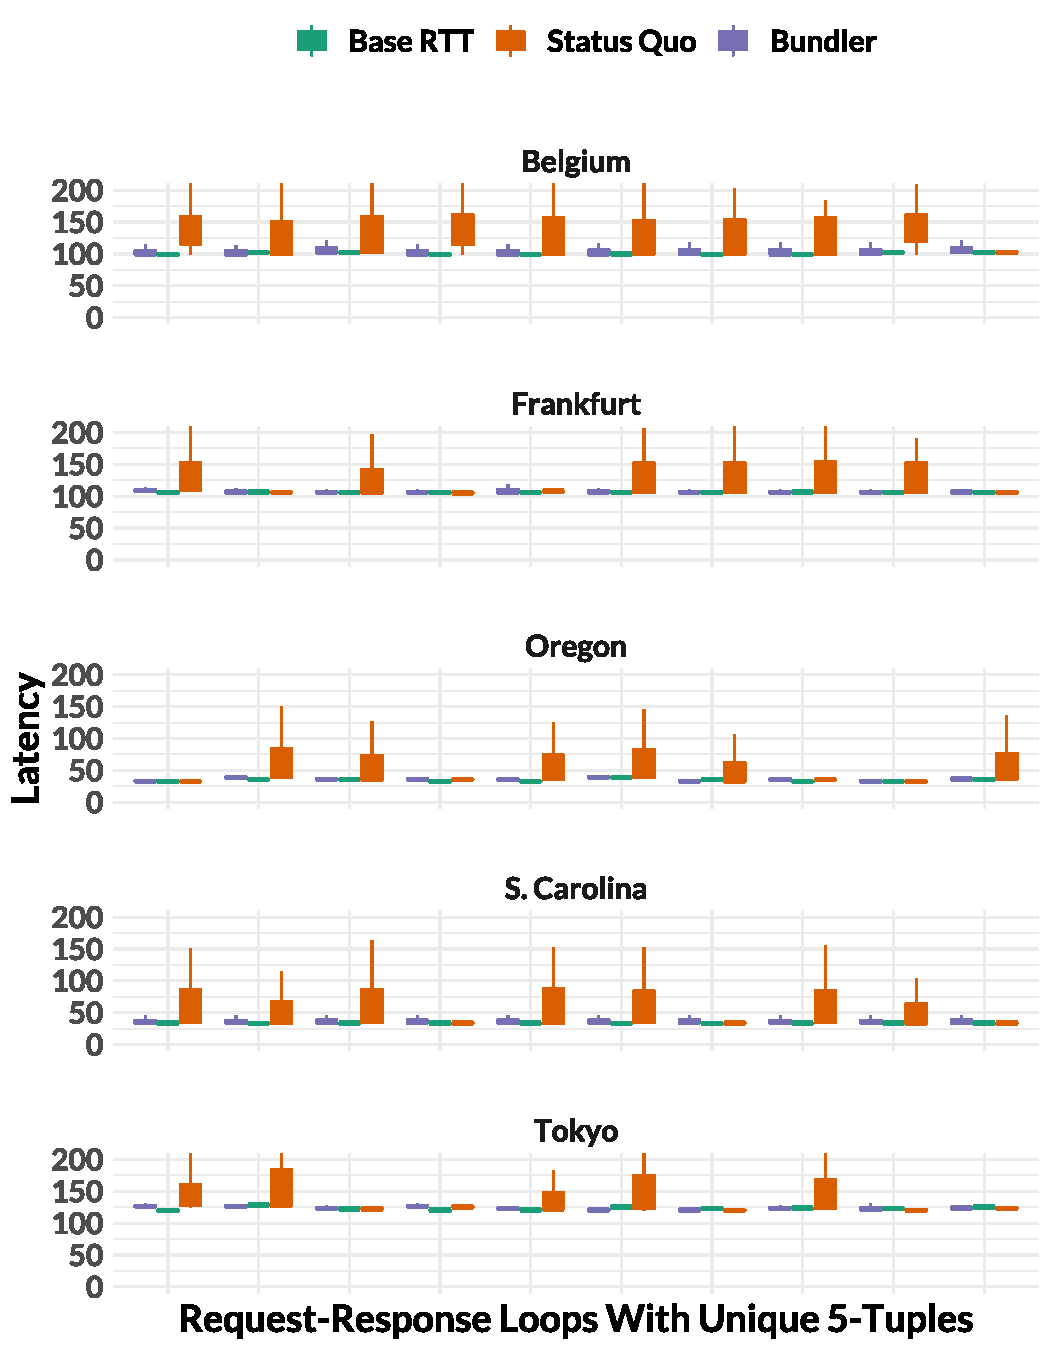
\includegraphics[width=\maxwidth]{figure/eval:realworld-1} 

\end{knitrout}
\newcommand{\realworldMedianLatencyImprovement}{57\%\xspace}
\newcommand{\realworldAvgBwRatio}{1\%\xspace}
\caption{On 5 real-Internet paths, \name achieves close to the Base RTT for latency-sensitive traffic. Each bar depicts an individual 5-tuple. Load-balancing in the Internet prevents queueing for some 5-tuples. \name still offers scheduling for paths with queueing (achieving \realworldMedianLatencyImprovement lower latencies overall) while achieving overall throughput within \realworldAvgBwRatio of that in the Status Quo scenario.}
    \label{fig:eval:realworld}
\end{figure}

\newcommand{\realworldMedianLatencyImprovement}{57\%\xspace}
\newcommand{\realworldAvgBwRatio}{1\%\xspace}
